\documentclass{article}
\usepackage{graphicx}
\begin{document}
\hfill Alejandro Chavez

\hfill Assignment 3 - Computer Architecture

\hfill \today\\

\begin{center}\begin{large}Digital Logic Chapter 3\end{large}\end{center}	Chapter 3
\begin{itemize}
	\item
		1)\\
	  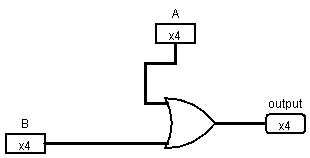
\includegraphics[scale=0.5]{assignment3bitwiseor.png}
  \item
		4)\\
	  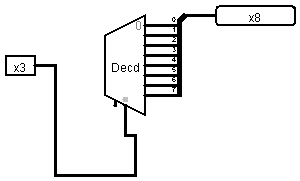
\includegraphics[scale=0.5]{assignment33to8decoder.png}
	\item
		5)\\

		\begin{tabular}{c|c}
    $A$ & $Out$ \\ \hline
    $000$ & $00000001$ \\
    $001$ & $00000010$ \\
    $010$ & $00000100$ \\
    $011$ & $00001000$ \\
    $100$ & $00010000$ \\
    $101$ & $00100000$ \\
    $110$ & $01000000$ \\
    $111$ & $10000000$ \\
		\end{tabular}\\
	
  \item
		6)\\
		$\overline{Sel}A\overline{B}+Sel\overline{A}B$
		\\Where A and B are 8 bit data paths and $Sel$ is a one bit data path selector.
	\item
		7)\\
	\begin{itemize}
		\item
			a)
			$10110111$
		\item
			b)
			$10111000$
		\item
			c)
			$01001000$
		\item
			d)
			$01001001$
	\end{itemize}
	\item
		8)\\
	  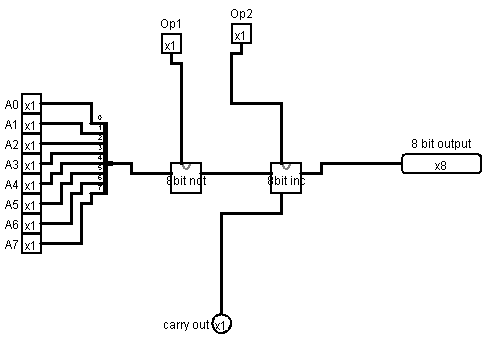
\includegraphics[scale=0.5]{assignment38bittinyalu.png}
	\item
		9)
		If ($Op_{2} == 00$) then $K_{2}$
		If ($Op_{2} == 01$) then $K_{2}+1_{2}$
		If ($Op_{2} == 10$) then $Inv. of K_{2}$
		If ($Op_{2} == 11$) then $(Inv. of K_{2})+1_{2}$
	\item
		10)
		You would need 2 bits, but only need three of the four permutations of the binary bits.\\
    
    \begin{tabular}{cccc|c}
    $A$ & $B$ & $C$ & $sel$ & $Out$\\ \hline
    $x$ & $y$ & $z$ & $00$ & $x$\\
    $x$ & $y$ & $z$ & $01$ & $y$\\
    $x$ & $y$ & $z$ & $10$ & $z$\\
    $x$ & $y$ & $z$ & $11$ & $undefined$\\
    \end{tabular}\\
		
	\item
		11) 3 select bits are needed for an 8 to 1 multiplexer. This multiplexer will contain an octal decoder.
	\item
		12) There is no problem 12.
\end{itemize}
\end{document}
